\documentclass[10pt]{beamer}

%STANDARD PREAMBLE
%https://tex.stackexchange.com/questions/68821/is-it-possible-to-create-a-latex-preamble-header
\usepackage{/Users/mwojno01/Research/Learning/latex_preamble/beamer_preamble}

%
%% ALLOW FOR ITEMIZE ENVIRONMENTS WITH NO PRECEDING
% SPACING, IF DESIRED
% Reference: https://tex.stackexchange.com/questions/86054/how-to-remove-the-whitespace-before-itemize-enumerate
%\usepackage{enumitem}% http://ctan.org/pkg/enumitem 
\usepackage{paralist}

\title{Bayesian Linear Regression}

\begin{document}

\maketitle

\begin{frame}{Bayesian Occam's Razor}
\scriptsize

\textit{Remember this slide?}

\begin{center}
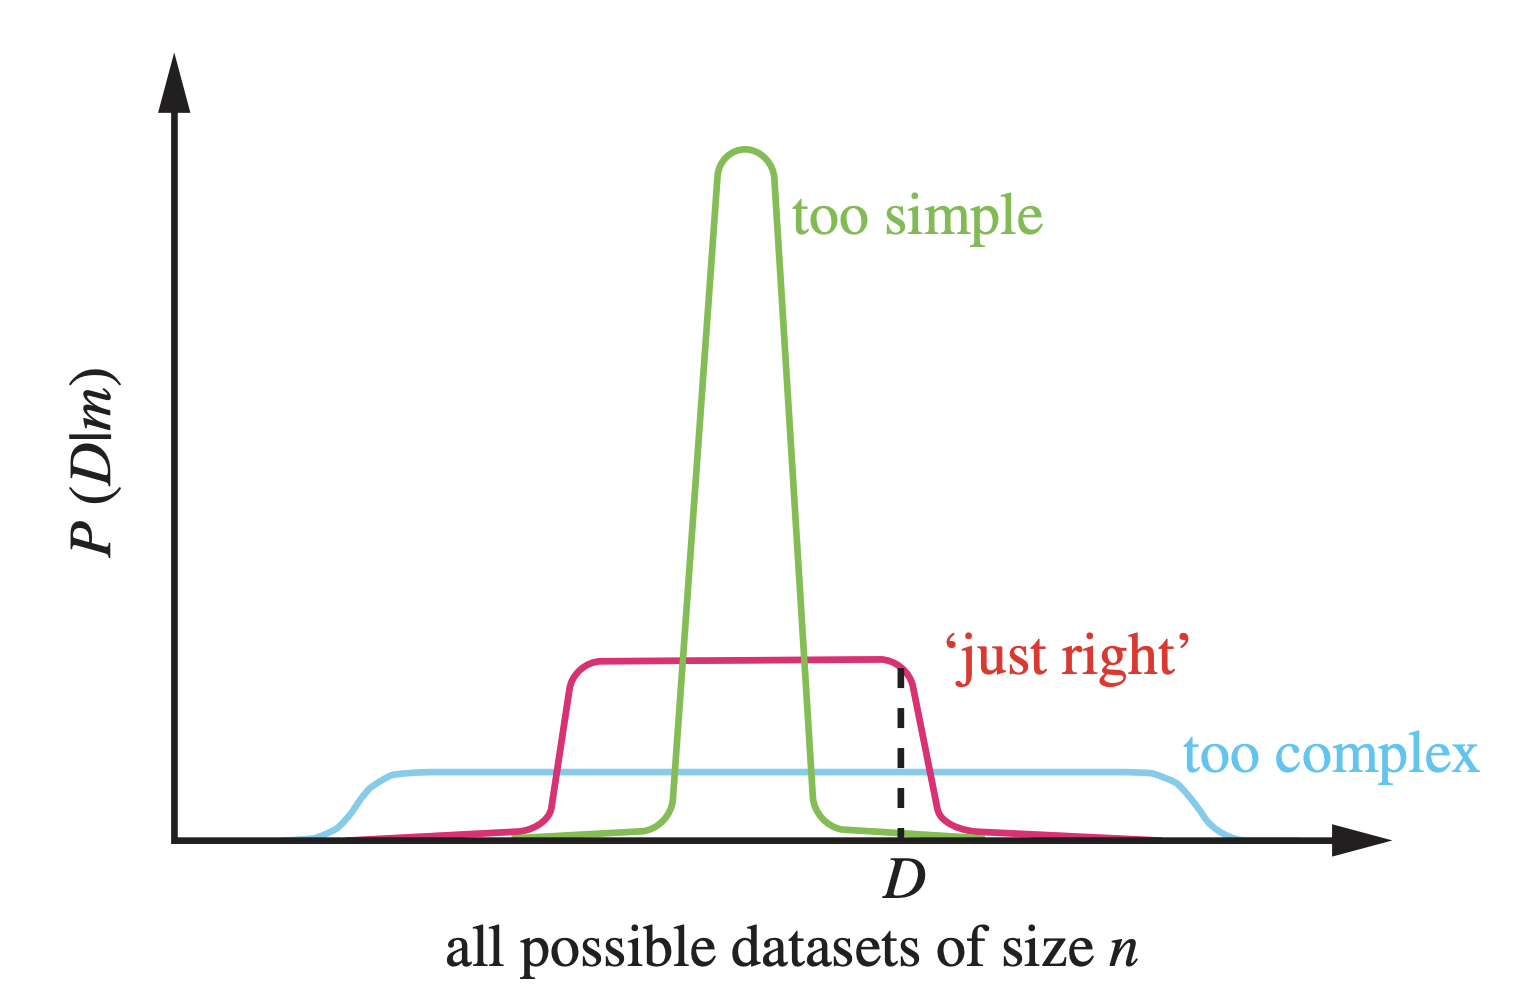
\includegraphics[width=.6\textwidth]{images/auto_occams_razor}
\end{center}
A \textit{complex} model (shown in blue) spreads its mass over many
more possible datasets, whereas a \textit{simple} model (shown in green) concentrates its mass on a smaller fraction of possible data.
Because probabilities have to sum to one, the complex model spreads its mass at the cost of not being able to model simple
datasets as well as a simple model—this normalization is what results in an automatic Occam razor. Given any particular
dataset, here indicated by the dotted line, we can use the marginal likelihood to reject both overly simple models, and overly
complex models. 


\hfill \tiny Ghahramani, Z. (2013). Bayesian non-parametrics and the probabilistic approach to modelling. Philosophical Transactions of the Royal Society A: Mathematical, Physical and Engineering Sciences, 371(1984), 20110553.
\end{frame}

\begin{frame}{Bayesian Occam's Razor}

{\scriptsize I generated $n=8$ data points from a \alert{cubic} distribution and used \texttt{NUTS} to fit Bayesian polynomials of various orders $p$.}

\vfill
    \begin{columns}
        \begin{column}{0.33\textwidth}
            %\centering %Uncomment this line for horizontal centering 
            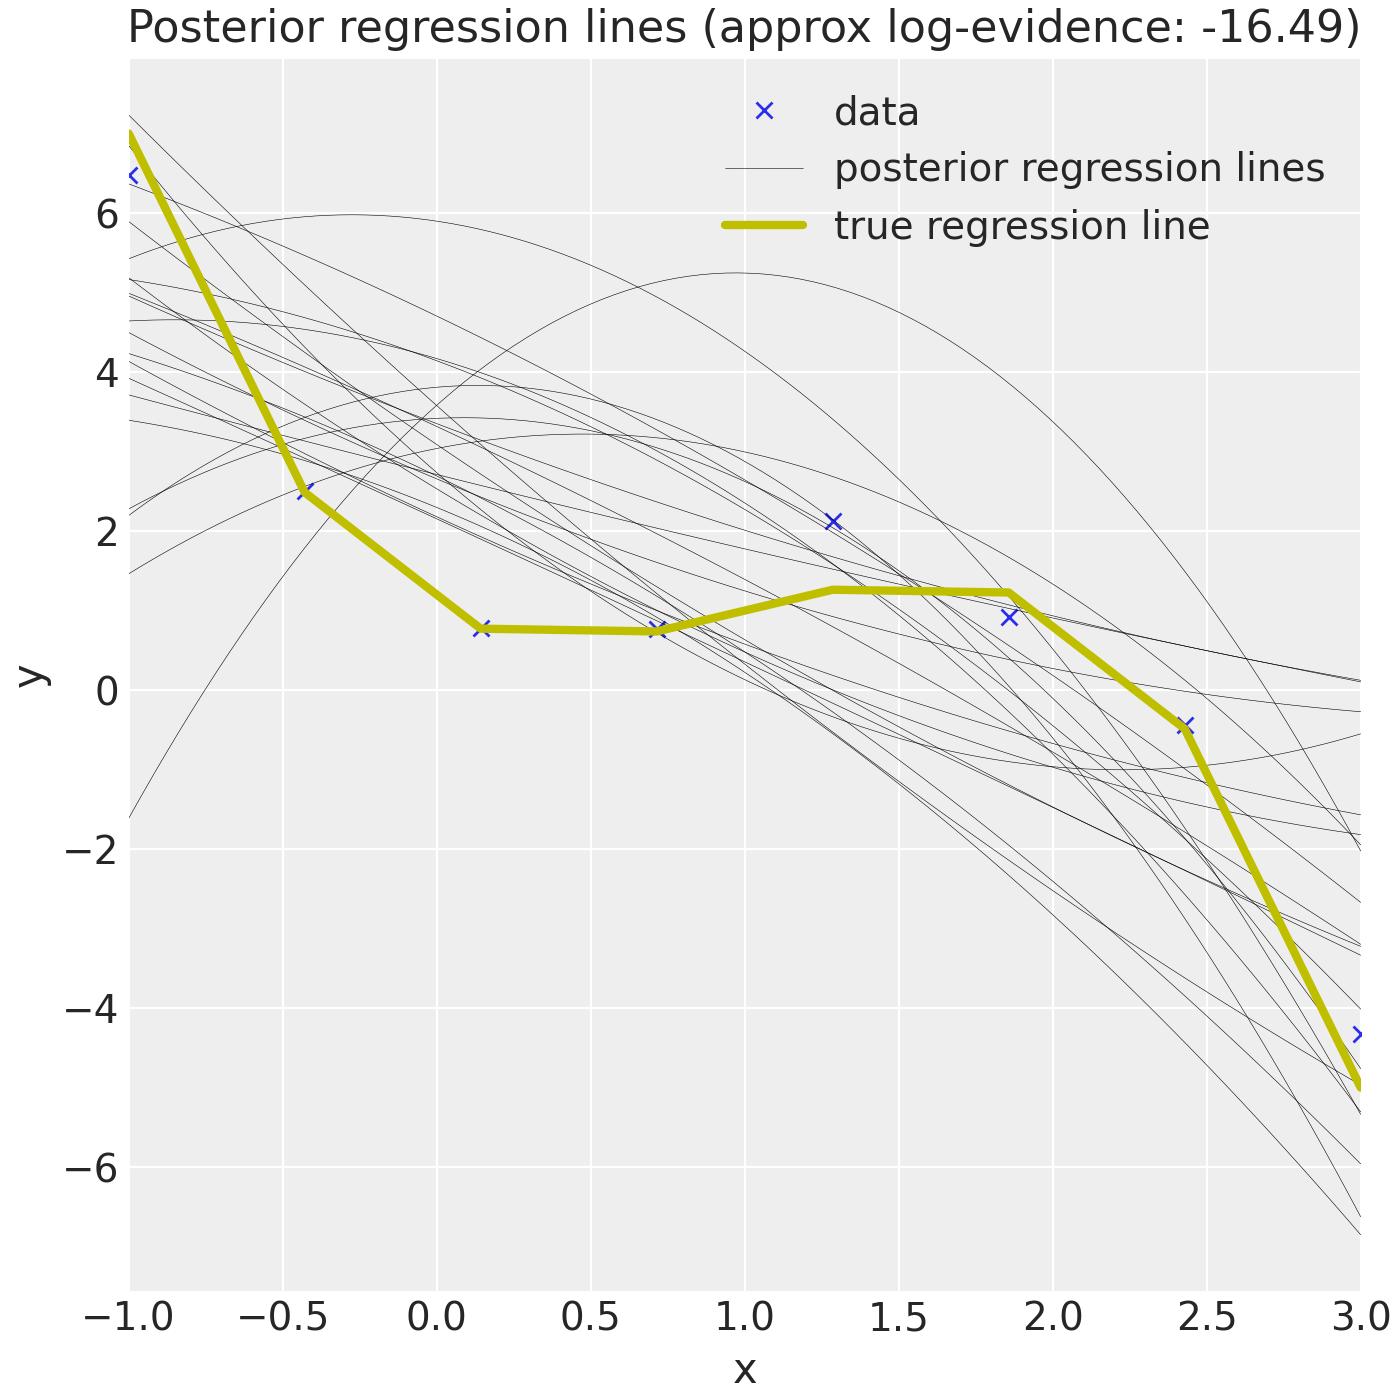
\includegraphics[width=\columnwidth]{images/bayesian_regression_quadratic_model}% \\
            
            Quadratic model ($p=2$)
        \end{column}
        \begin{column}{0.33\textwidth}
            %\centering %Uncomment this line for horizontal centering 
            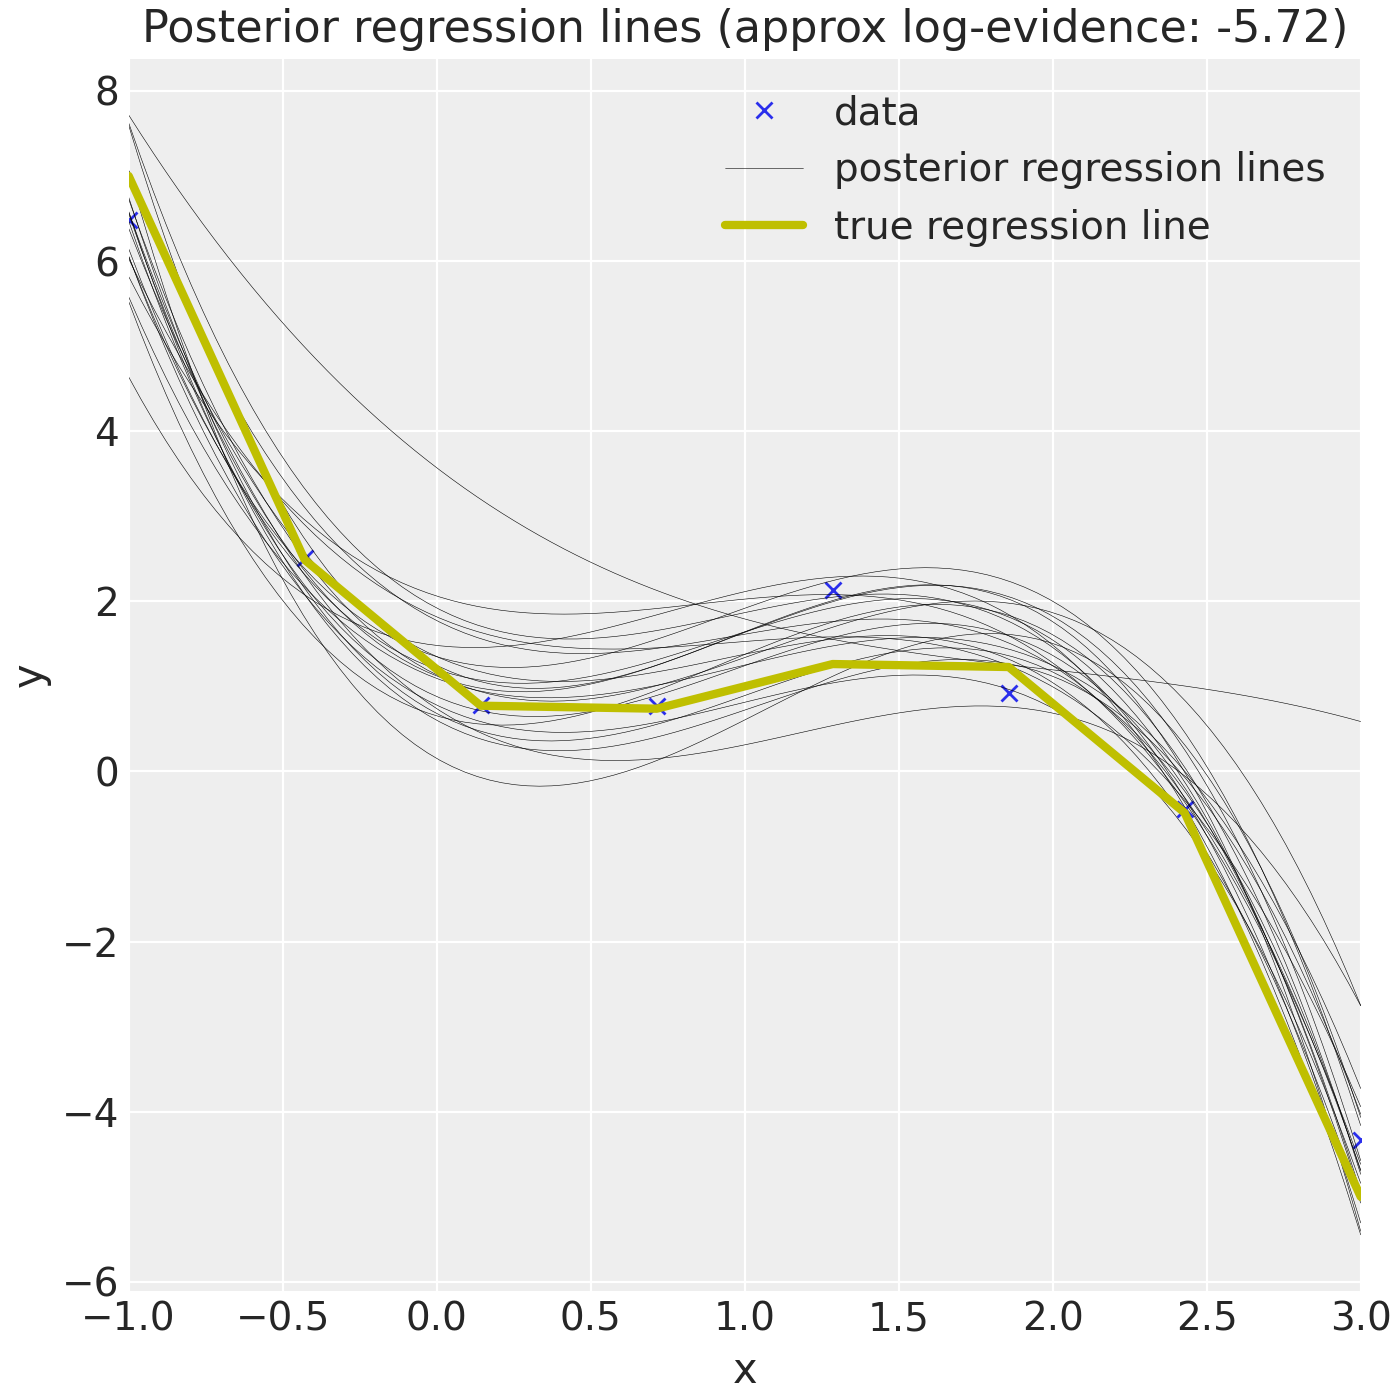
\includegraphics[width=\columnwidth]{images/bayesian_regression_cubic_model}%\\
            
            Cubic model ($p=3$)
        \end{column}
        \begin{column}{0.33\textwidth}
            %\centering %Uncomment this line for horizontal centering 
            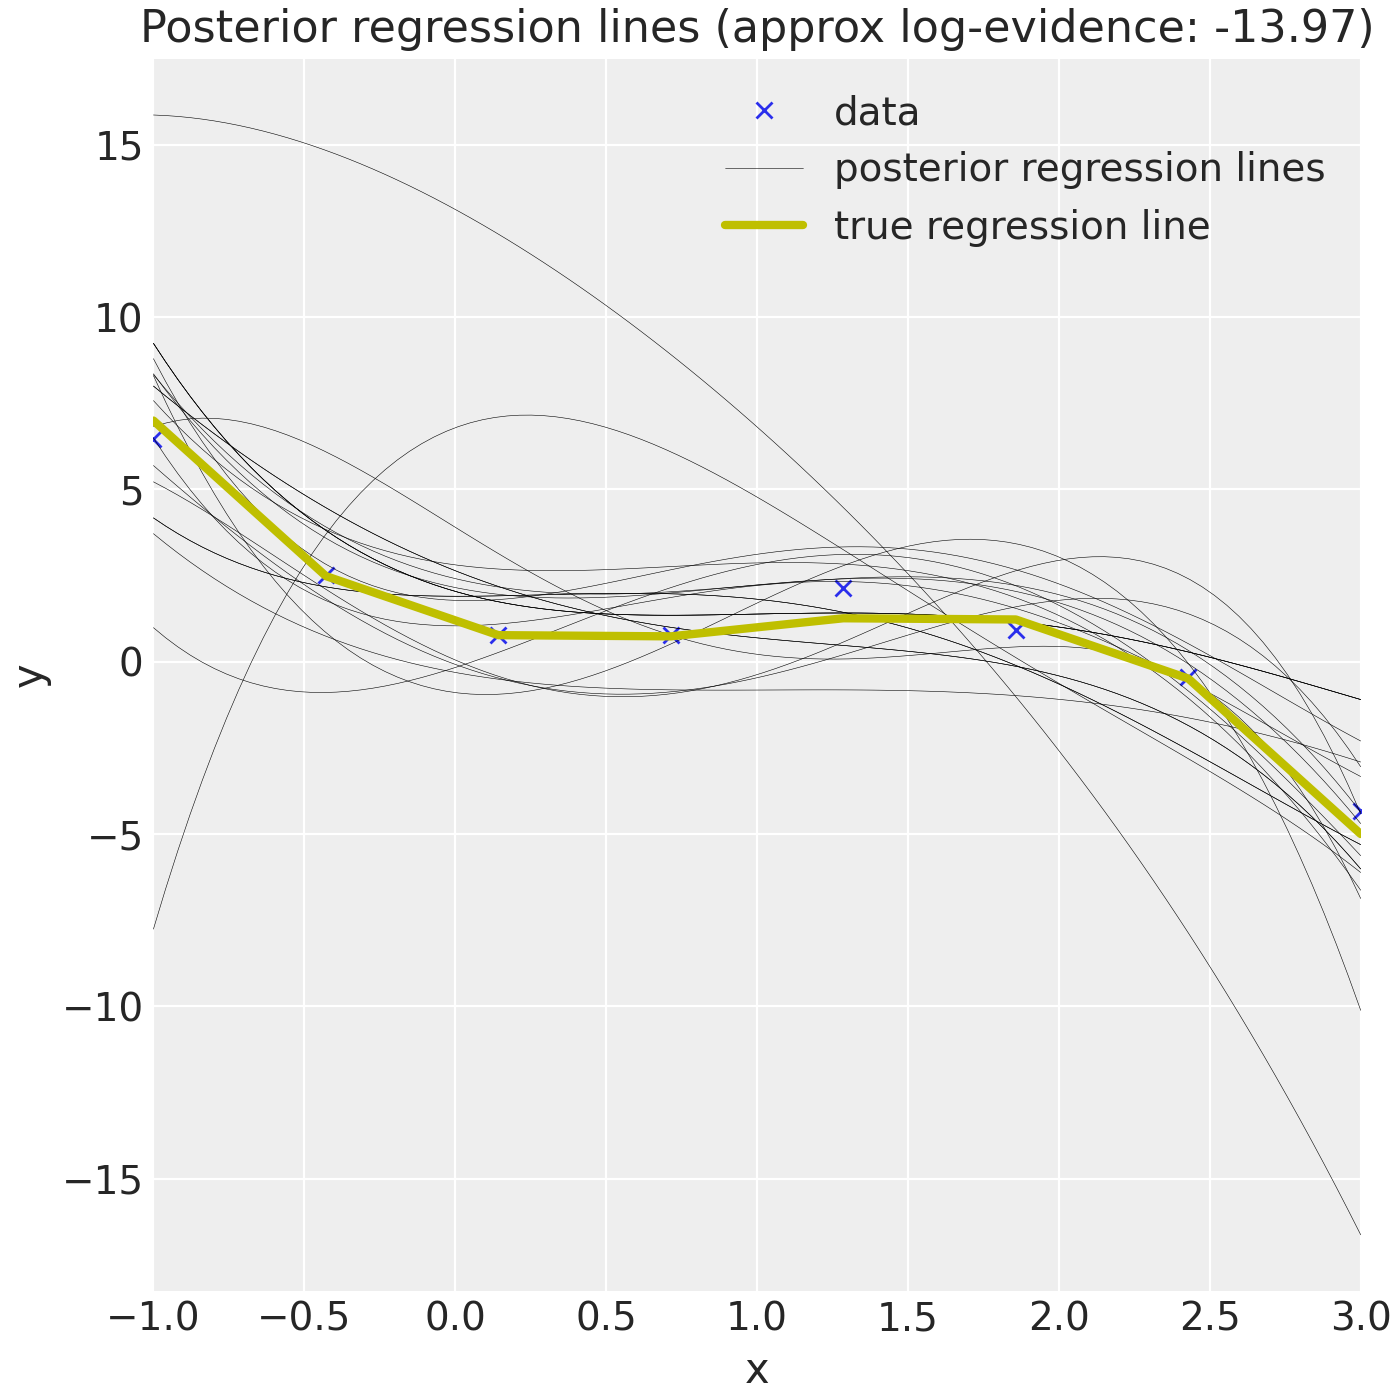
\includegraphics[width=\columnwidth]{images/bayesian_regression_fourth_order_model}%  \\
            
              Quartic model ($p=4$)
        \end{column}
    \end{columns}

\vfill 

{\scriptsize
\textbf{Observations} \pause 
\begin{itemize}
\item Bayesian model selection works well here!  The true (cubic) model has the highest evidence.  The evidence is lower for models that are underfit (quadratic) or overfit (quartic).
\item Correspondingly, typical draws from the posterior model best match the true data generating process.
\end{itemize}
}

\end{frame}


\end{document}